\section{Выбор инструментальных средств}

\subsection{Выбор микроконтроллера}
Основными требованиями предъявляемыми мной к центральному вычислительному устройству создаваемого устройства является:
\begin{itemize}
	\item{} Не высокая стоимость.
	\item{} Низкое энергопотребление
	\item{} В число доддерживаемой переферии должен присутствовать ЦАП. 
	\item{} Необходимо наличие аппаратной поддержка SPI
	\item{} Поддержка производителем этого рода устройств.
	\item{} Доступность устройства.
	\item{} <<Сильное>> сообщество разработчиков под эту архитектуру.
	\item{} <<Наличие книг>>
\end{itemize}

По всем этм пунктам идеально подходят микроконтрллеры серии XMega компании ATmel.

Микроконтроллеры серии XMega обладают следующими характеристиками:
\begin{itemize}
	\item{} 8/16-битное высокопроизводительное RISC ЦПУ AVR;
	\item{} 138 инструкций;
	\item{} аппаратное умножающее устройство;
	\item{} 32 8-битных регистра, напрямую подключенные к АЛУ
	\item{} прямая адресация до 16 Мбайт памяти программ и 16 Мбайт памяти данных;
	\item{} полная поддержка 16/24-битного доступа к 16/24-битным регистрам ввода-вывода;
	\item{} эффективная поддержка 8-, 16- и 32-битных арифметических инструкций;
	\item{} защита от изменения настроек критических функций системы.
\end{itemize}

\begin{figure}[h]
	\center{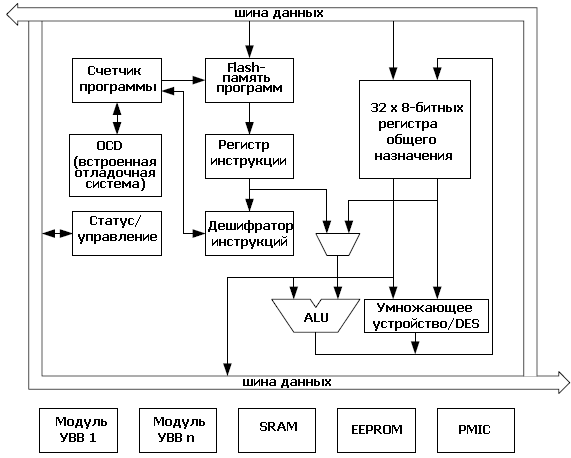
\includegraphics[bb=0 0 360 290]{avr_arch.png}}
	\caption{Архитектура AVR}
	\label{img:avr_arch}
\end{figure}

В целях достижения максимальной производительности и параллелизма у МК AVR используется Гарвардская архитектура с отдельными памятью и шинами программ и данных. Инструкции, хранящиеся в памяти программ, выполняются на одноуровневом конвейере. Это означает, что во время выполнения одной инструкции выполняется предварительная выборка из памяти программ следующей инструкции. Данная концепция делает возможным выполнение по одной инструкции за каждый цикл синхронизации.



\subsection{Язык программирования микроконтроллра}
Микропрограммы для микроконтроллеров XMega можно писать на нескольких языках программирования.
Сама компания Atmel предоставляет для программирвания своих устройств два средства разработки:
	\begin{enumerate}
		\item{}AVR Assembler
		\item{}AVR-Gcc --- кодогенератор и набор дополнительных утилит для Gnu C Compiller от компании Atmel, активно поддерживаемый сообществом разработчиков, а так же входящий в комплект среды разработки AVRStudio, AVR32Stdio, MacAVR, и распростроняемый на правах свободного программного обеспечения.
	\end{enumerate}

TODO






\subsection{Выбор EDA системы}
TODO

\subsection{Выбор языка программирования сетевого сервиса}

При проектировании сетевого сервиса от инструментального средства требуется что бы оно отвечало следующим требованиям [Профессиональное программирование. Системный подход. Одинцов В., BHV-СПб 2004]:

\begin{enumerate}
	\item{} Инструментальное средство должно быть высокого уровня --- язык высокого уровня, освобождает разработчика от рутинной работы вроде ручного выделения и освобождения памяти, и позволяет ему сфокусироваться на оперировании абстракциями предметной области.
	\item{} Язык должен минимизировать количество ошибок которые может допустить программист в процессе разработки системы.
	\item{} Высокая степень параллелизма --- необходима возможность обслуживать тысячи клиентов одновременно.
	\item{} Отказоустойчивость --- телеком-системы слишком масштабны, чтобы самому разработчику имело смысл даже пытаться предусмотреть все возможные ошибки.
	\item{} Возможность обновления кода сервиса без останова выполнения программы.
	\item{} Наличие обширной системной библиотеки,  а так же предопределённых каркасов  проектов --- это избавляет разработчика от необходимости реализовывать типовые решения самостоятельно, при этом тратя время на тестирование и отладку системы. Каркас проекта задаёт общую структуру создаваемой системы, что позволяет ещё на этапе проектирования системы оценивать её будущие качества.
\end{enumerate}

\begin{par}
Один из немногих существующих и поддерживаемых на сегоднешний день языков программирования отвечающих всем этим требованиям является Erlang и платформа Open Telecom Platform (OTP).
\end{par}

\subsubsection{Обзор языка Erlang и платформы OTP}

\begin{par}
В середине 1980-х, Ericsson Computer Science Laboratory было дано задание --- исследовать языки программирования подходящие для разработки телекоммуникационных продуктов нового поколения. Джой Армстронг(Joe Armstrong), Роберт Вирдинг (Robert Virding) и Майк Вильямс (Mike Williams) под руководством Брайна Декера (Bjarne Dacker) потратили два года на прототипирование телекоммуникацинного приложения поочерёдно  используя все доступные на тот момент языки и системы программирования. В результате, несмотря на то, что многие языки программирования обладали интересными и подходящими свойствами, ни один из них не удовлетворял всех их требованиям. В результате они приняли решение создать их собственный язык программирования.
\end{par}

\begin{par}
Erlang был создан под влиянием  функциональных языков таких как  ML и Miranda, параллельных языков ADA, Modula и Chill, и языка логического программирования Prolog. Erlang так же унаследовал некоторые черты таких язков как Smalltalk, проприетарных языков Ericsson EriPascal и PLEX.
[Erlang programming - by Francesco Cesarini and Simon Thompson, O'Reilly, 2009]
\end{par}

\begin{par}
Используя построенную на Prolog виртуальную машину Erlang (VM), лаборатория потратила  четыре года на прототипирование телекоммуникационного приложения с применением и постоянными доработками новго языка. Именно из-за применения метода проб и ошибок язык Erlang стал таким, каким он является сейчас. В 199 Майк Вильямс переписал на Си виртуальную машину, и годом позже, на этом языке был выпущен первый коммерческий продукт. 
\end{par}

\begin{par}
История создания языка Erlang важна для понимания его философии, так как в отличии от других языков, которые находили свою нишу уже после разработки и распространения, Erlang изначально создавался для решения конкретных задач бизнеса. Он создавался под задачи построения распределённых, отказоустойчивых систем реального времени массового обслуживания.
\end{par}

\begin{par}
Так как такие области как системы поддержки продаж, банковские системы, системы компьютерной телефонии, системы интеграции уровня предприятий зачастую предъявляют к своему программному обеспечению аналогичные требования, то Erlang нашёл своё применение и в них.
\end{par}

Подтверждением применимости Erlang в этих областях могут служить факты использования этого языка в проектах компаний:
\begin{itemize}
	\item{} Amazon --- использует Erlang для реализации SimpleDB, предоставления системы управления базами данных как части Amazon Elastic Compute Cloud (EC2).
	\item{} Yahoo! --- использует Erlang для реализации своего сервиса социальных закладок, который обслуживает более 5 милионов пользователей и 150 милионов URL.
	\item{} T-Mobile --- использует Erlang в их SMS и авторизирующей системах.
	\item{} Motorola --- использует Erlang в системе обработки звонков системы обслуживания клиентов.
	\item{} Ericsson --- использует Erlang для поддержки узлов используемых в GPRS и 3G мобильных сетях по всему миру.
	\item{} Facebook и Yandex --- используют написанный на Erlang сервер мгновенных сообщений Ejabberd.
\end{itemize}
